\documentclass[10pt,twocolumn,letterpaper]{article}
\usepackage{cvpr}
\usepackage{times}
\usepackage{epsfig}
\usepackage{graphicx}
\usepackage{amsmath}
\usepackage{amssymb}
\usepackage{graphicx}
\graphicspath{ {./images/} } 
\usepackage{subfig}
\usepackage[pagebackref=true,breaklinks=true,letterpaper=true,colorlinks,bookmarks=false]{hyperref}
\usepackage{subfig}
\cvprfinalcopy 
\def\httilde{\mbox{\tt\raisebox{-.5ex}{\symbol{126}}}}
\ifcvprfinal\pagestyle{empty}\fi
\begin{document}
\title{\Ensuring Ensuring lock-down in COVID 2019 with help of still CCTV and UAVs\ }
\author{Avani Gupta\\
IIIT Hyderabad\\
Gachibowli\\
{\tt\small avani.gupta@research.iiit.ac.in}

\and
}
\maketitle
\begin{abstract}
    During the Pandemic of COVID 19,ensuring social distancing to flatten the curve and prevent the disease from spreading is the only way to stop it. lock-downs help to ensure this very effectively.
     Police is working day and night to cater to those people and penalize the breakers. But police task forces being on ground does hamper the purpose of lock-down. This paper presents a Computer Vision and Robotics based solution which involves object tracking and face recognition to cater this situation. The solution presented here, makes use of live CCTV footage and  autonomous Unmanned Aerial Vehicles UAV's  for monitoring of lock-down breakers and a  web-app which acts on police's end and helps penalise lock-down breakers. We also have a app at users end where he can report lock-down violation in his locality.

\end{abstract}

\section{Introduction}

Social distancing to flatten the curve \cite{thunstrom2020benefits} has been proved crucial to prevent the virus from spreading. \cite{block2020social}
    lock-downs have been quite effective to implement social distancing, many countries including India are announcing lock-downs. India experienced a lock-down of 21 days which later got extended to 42 days. There are many people who still can't understand the seriousness of the situation and break lock-downs. Police is working day and night to cater to this situation and penalize the lock-down breakers. Police officials risk their own  lives to ensure the safety of entire nation. But police task forces being on ground does hamper the purpose of lock-down along with risk of spread among the policemen. Many policemen have even lost their lives due to becoming positive on duty hereby becoming "Corona Warriors". \\
    With advancements in computer vision, aerial robotics, and reinforcement learning based control for autonomous drones it is possible to detect the law-breakers with cameras and hence ensure lock-down. \\
    Another point being, police taskforce is limited and it is difficult to determine all cases of lock-down violation. 
    The use of face detection algorithms and UAV's can increase efficiency of detection , and help police track the violation without themselves being on field. \\
    This paper presents a methods for enhancing closed-circuit television (CCTV) systems by using face detection and object detection for real time detection and tracking of people breaking lock-down. We also use using autonomous unmanned aerial vehicle (UAV)also known as drones fitted with CCTV's  for surveillance.
    
%-------------------------------------------------------------------------

%------------------------------------------------------------------------
\section{Literature Review}

Police in India has been using remote controlled drones to monitor the lock-down. There are advancements in Reinforcement Learning based autonomous drones used for surveillance of surroundings \cite{pham2018cooperative}.
\subsection{Face Detection}
Also with advancements in Computer Vision it is possible to detect the person from the face detection techniques. Viola Jones algorithm \cite{viola2001robust} makes use of Haar Features which is based on similarity among human faces. Some of the Haar- features include:
\begin{itemize}
\item Property of Human faces like eye region is darker than the upper-cheeks and nose bridge region is brighter than the eyes
\item Composition of properties forming match-able facial features like Location and size of eyes, mouth, bridge of nose and oriented gradients of pixel intensities.
\end{itemize}

 FaceNet \cite{schroff2015facenet}is a popular method for face detection which uses a mapping from face images to a compact Euclidean space where distances directly correspond to a measure of face similarity.Now, FaceNet embeddings can be used as feature vectors for face identification. It uses a deep convolutional network which optimizes the embedding.

\subsection{Drone surveillance } 
\subsubsection{Usage in journalism} 
There are studies for using the  drone surveillance in journalism for reporting \cite{gynnild2014robot}. They are used to gather videos and live report of in-accessible areas. \\
\subsubsection{Real-time Traffic Monitoring} 
 UAVs are also being used for real-time Traffic Monitoring \cite{8377077}. They help by keeping track of trajectories, behaviors and vehicle types. As stated in \cite{8377077}, UAV's are equipped with image processing and collect various information like vehicle position, speed, and direction, the number of vehicles within an area, the number of vehicles passing through a given point etc.\\
 \subsubsection{Optimising number of UAV's required} 
 Number of UAV's needed to cover a particular area can be optimised by making target clusters by taking in velocities of vehicles and distance to be covered and assigning a cluster to every UAV. UAV trajectories are guided by predefined Points Of Interest(points with high traffic). \cite{1618950} and multiple cooperative UAV's. The multiple UAVs are capable of of identifying the targets in their FoV and estimating their positions and speeds, and exchange those information between each other and with a central point. UAVs trajectories are adaptive and POIs are mobile. They use kinematics eg: knowledge of Center of Gravity of their groups of targets to fly over the computed positions and adjust their velocities according to their targets. \\
 
 \subsubsection{Trajectory planning}
  Shortest Path Map-Based Movement model is used to guide the trajectory of the UAV so that it moves exactly above roads, and do observation regarding the targets in their FoV. \\
\subsubsection{Real time Surveillance of People: Detection and Identification}  
  Drones are used for real time tracking of people \cite{8692269}. \cite{8692269} used Haar-cascade classifier and max-margin object detection with convolutional neural network based features for face detection and color detection system for
obstacle detection. They use image processing and machine learning to control the UAV automatically. They do tracking by calcuating Region of Interest using centroid which is calculated using pixel positions on axes and move drone by comparing the size of ROIs. If ROI is higher than threshold the drone is moved foward, else backward.

The distances from drones and their targets directly affect
the size of the facial images in pixels. Since drones take picture from the air, altitudes of drones keep them distant from their targets on the ground. 
shows that augmenting 3D information captured by drone camera helps to
boost face recognition performance in the case of large angles of
depression. It uses Face++ and ReKognition which provides an open API for development of various kinds of applications.
\subsubsection{Full coverage of Field by multiple UAV's by Reinforcement Learning}
Multi-Agent Reinforcement Learning (MARL) algorithm \cite{ham2018cooperative}allows UAVs to learn cooperatively to provide a full coverage of an unknown field of interest while minimizing the overlapping sections among their field of views. 
\cite{opencv_library} 
%-----------------------------------------------------------------------
\section{System Architecture}
We propose the architecture with real time detection and tracking of people. We use Haar-cascade classifier along with facenet embedding and max-margin object detection with convolutional neural network  for face detection and object detection. \\
The system would act as a replacement for police surveillance, we use CCTV fitted on streets and UAV's for this. All areas under lock-down or special red-zones(hotspots) are tracked using drones and all other ares are tracked using CCTV's installed in streets. Now, when a person is seen on street, he is asked by the system fitted on streets for the reason of coming out (from home using Natural Language processing) if his reason is a valid reason(checked using Artificial Intelligence) he is allowed to proceed, if not, he is alerted to go back to home. Starting from his home he is tracked by cameras(with no deterrent to privacy) if he does'nt go home, the system sends a message of fine to his phone number. \\

 \begin{figure}
    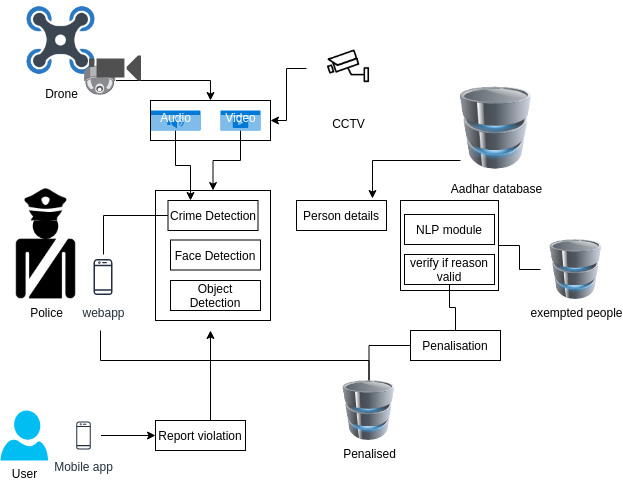
\includegraphics[width=.5\textwidth,height=.4\textheight,keepaspectratio]{images/componets.png} 
      \caption{Components}
\end{figure}

 \begin{figure}
    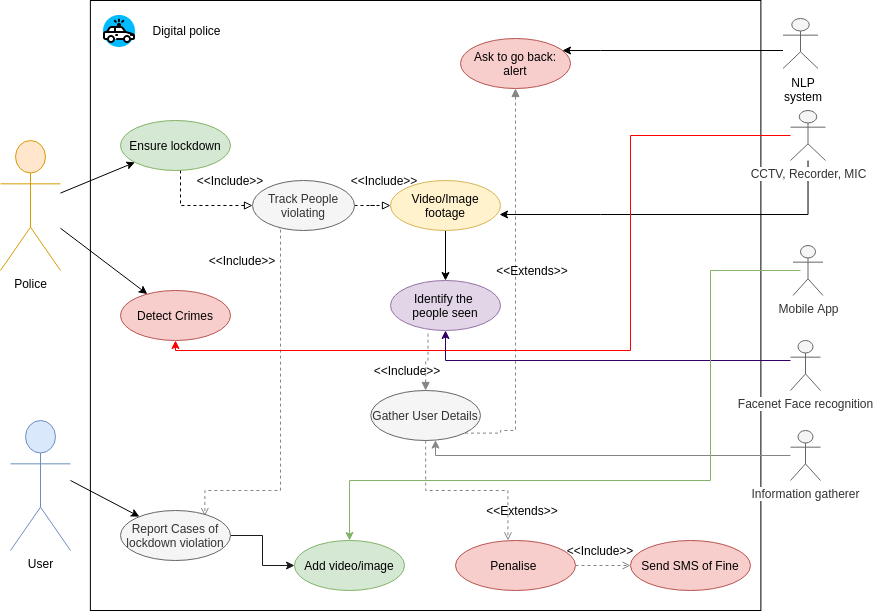
\includegraphics[width=.5\textwidth,height=.8\textheight,keepaspectratio]{images/usecase_diagram.png} 
      \caption{Use case diagram}
\end{figure}
\subsection{Major Functionalities}
\subsubsection{Capture Footage}The video, audio of locations is recorded by CCTV's fitted on streets and drones.
\subsubsection{Real time tracking path} The real time tracking of the path followed by people coming outside in lock-down is traced by drones street cameras and using object detection and path detection.
\subsubsection{Detecting People}The person is identified using face detection algorithm which uses Haar-cascade features along with facenet embedding for face detection. It is connected to Aadhar card database by government. The database is searched for image of person and identification is done. 
\subsubsection{Asking reason of Travel} Now, the moment the person comes out from home, he is asked for the reason of travel by the AI (using Natural Language processing through a speaker)
\subsubsection{Saving information of people who have a permanent need of travel}
\subsubsubsection{Identifying police and doctors automatically} Ambulance, doctors, policemen are excepted automatically and are not asked for prompt by NLP module. They are identified using a trained classifier on videos and images of those.
\subsubsubsection{Saving information of other essential services people} It is a smart system which saves the information of people who have valid reason of travel, Journalists, those connected with essential services like vegetables, groceries etc apart from doctors, nurses, policemen and doesn't ask those people any reason for travel.
\subsubsection{Communication among all systems}
If even after prompt the person does'nt go back(or tries to fool the system by turning back and taking different route, he can't. Here comes the most effective part of system. The systems communicate among themselves(all data shared among various UAV's and CCTV's). So the person is tracked until he goes home.
\subsubsection{Message for Fine}
\begin{itemize}
\item If a person does not follow the instruction alert, he is immediately sent a message for fine on his phone number.
\item If a person follows but is found again without a valid reason he is sent a fine.
\end{itemize}
\subsubsection{Maintaining Social Distancing}
If a group of people found going together even with a reason they are alerted to follow social distancing norms.
\subsubsection{Crime Detection} Crime is detected in the audio/ video and location is sent to the police.
\subsubsection{Signal processing}
The system detects crimes  using  signal processing of audio to identify fighting  and image processing to detect an intruder.
\subsubsection{Alert Police: Alert alarm on phone}
The nearby police station is alerted about a crime through an alert alarm and message on a mobile app on policeman's phone.

\subsection{Different Modules}
\subsubsection{Face Detection} 
We use Haar-cascade classifier along with facenet embedding for real time Face Detection.
\subsubsection{Object Detection} 
Detecting various objects in Video/ image. We use max-margin object detection with convolutional neural network for object detection.
\subsubsection{Natural Language Processing Module along with audio signal Processing} 
For asking the user the reason of travel and processing his answer, we use Natural Language Processing which is combined with audio signal processing to track what user says.
Mic and recorder fitted in drone and near CCTV in streets used to interact with the person.
\subsubsection{Drone Control} 
The Drone control is based on several parameters.
\begin{itemize}

\item \textbf{\emph{ Reinforcement Learning based Control}}\\
We propose a Reinforcement learning based control which makes use of asynchronous methods of continuous control through DDPG, TRPO and PPO algorithms\cite{article}
\item \textbf{\emph{Optimising number of UAV's required}}
Number of UAV's needed to cover a particular area can be optimised by making target clusters as cited in  \cite{1618950}.

\item \textbf{\emph{Communication among systems}}
There is a communication among various drones as well as CCTV's fitted at different locations. They notify other systems with a range when lock-down is violated and convey the location and path of the person who violated lock-down. 
\end{itemize}
\subsection{Crime Detection}
There is a sudden outburst of sound when a crime occurs. the energy of sound signal during fighting is higher than when in normal situation and the change pixel is increased when there is an intruder \cite{6704220}. This property is used to detect crimes in a locality through audio and video.
\subsection{Webapp at police's end}
The web-app at Police's end is used to alert the police in case of crime Detection

\subsection{Information Gatherer}
The information gather is connected to Aadhar Database and gathers all information about the lock-down breaker and criminal.
Also it store the voilation history and penalized data of people which is displayed to police to web-app if required.

\subsection{Mobile App for Users}
A common person can report the lock-down voilation through the mobile app by uploading the image and video.
 \begin{figure}
    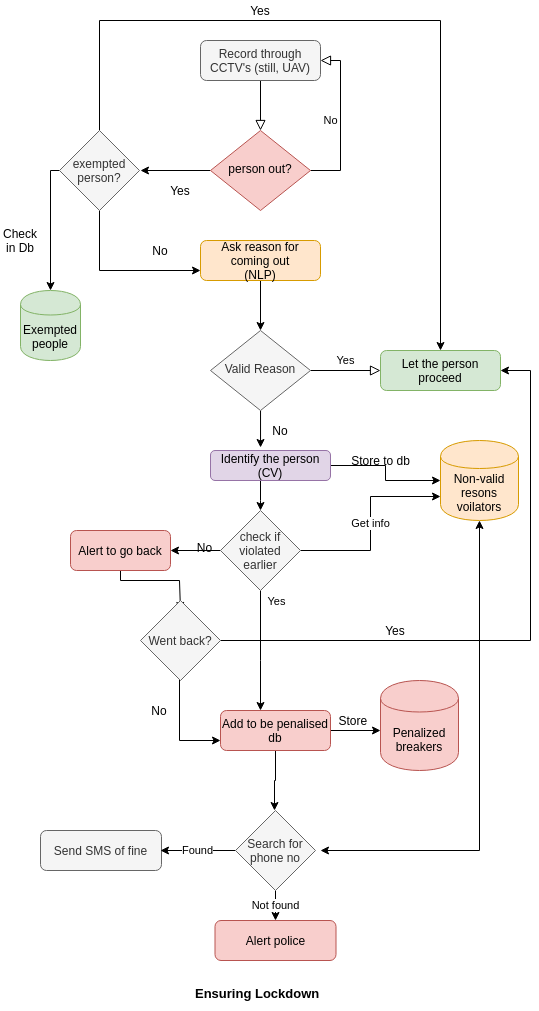
\includegraphics[scale=0.45]{images/general_flow.png} 
  
    \caption{General flow}
    
\end{figure}
 \begin{figure}
    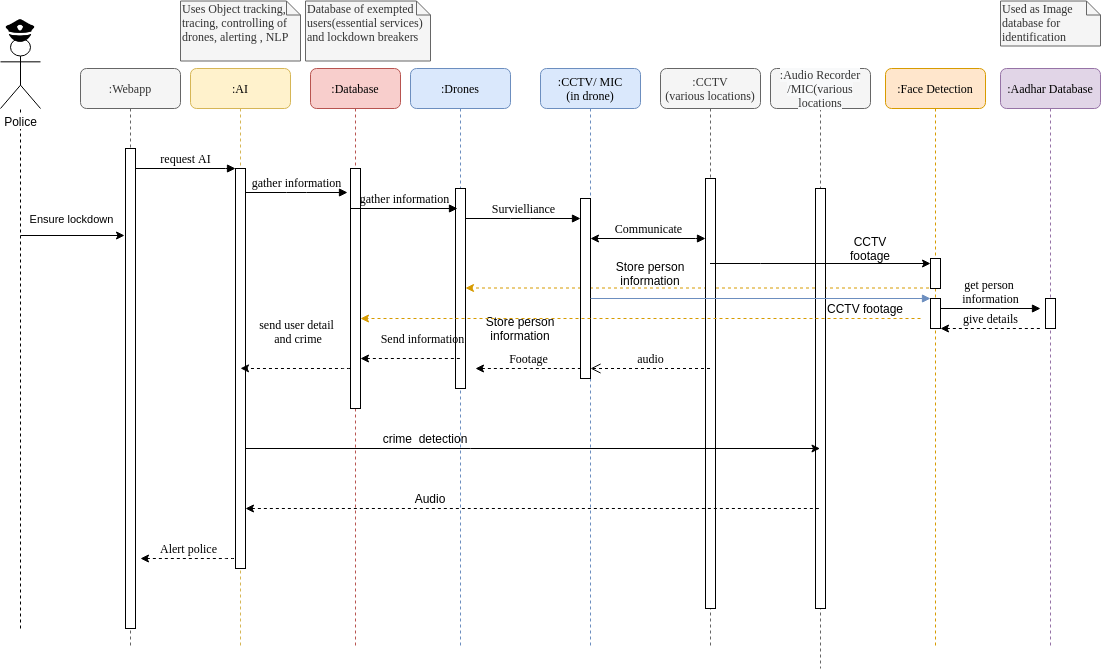
\includegraphics[height=.45\textwidth, width=.55\textwidth]{images/sequence_diagram.png} 
   
    \caption{Sequence Diagram}
\end{figure}
 \begin{figure}
    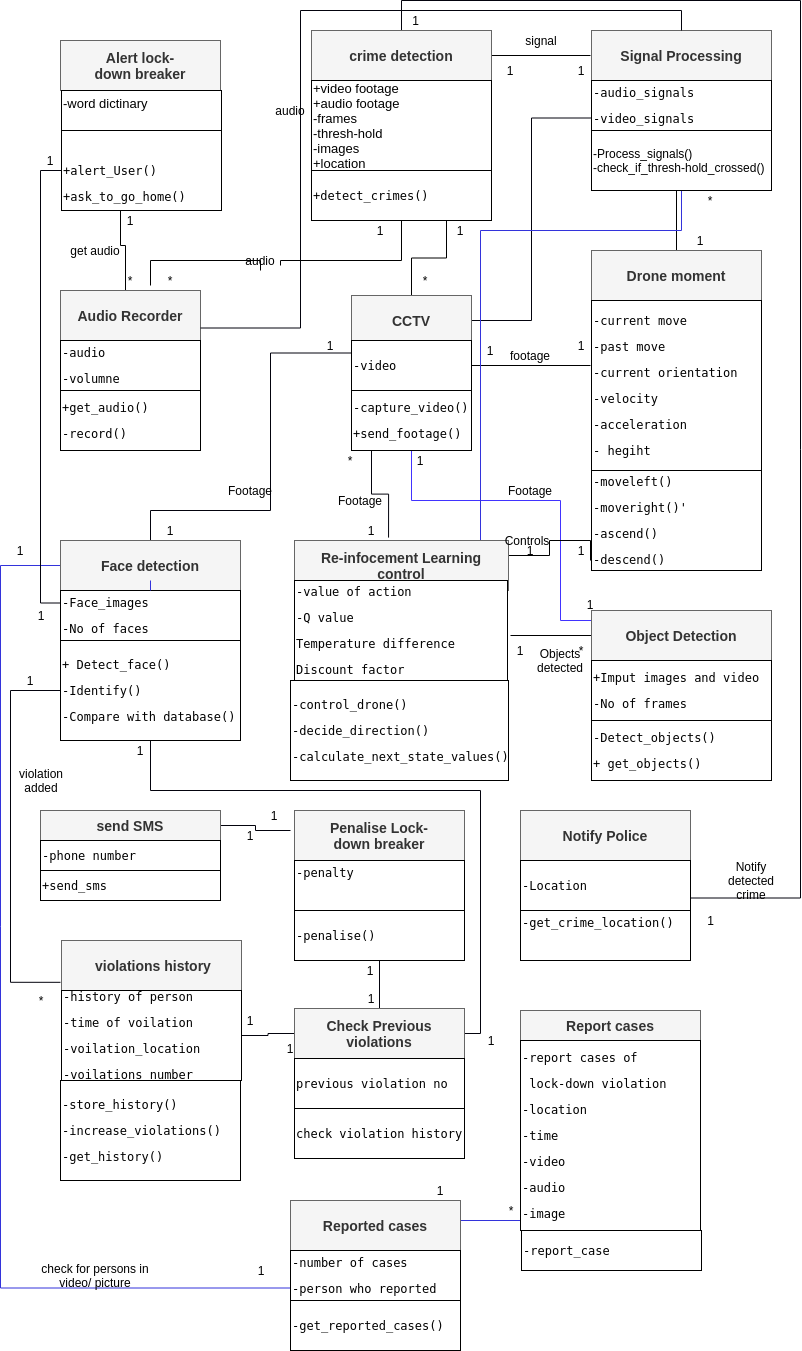
\includegraphics[height=.7\textwidth, width=.55\textwidth]{images/class_diagram.png} 

    \caption{Class Diagram}
\end{figure}
 \begin{figure}
    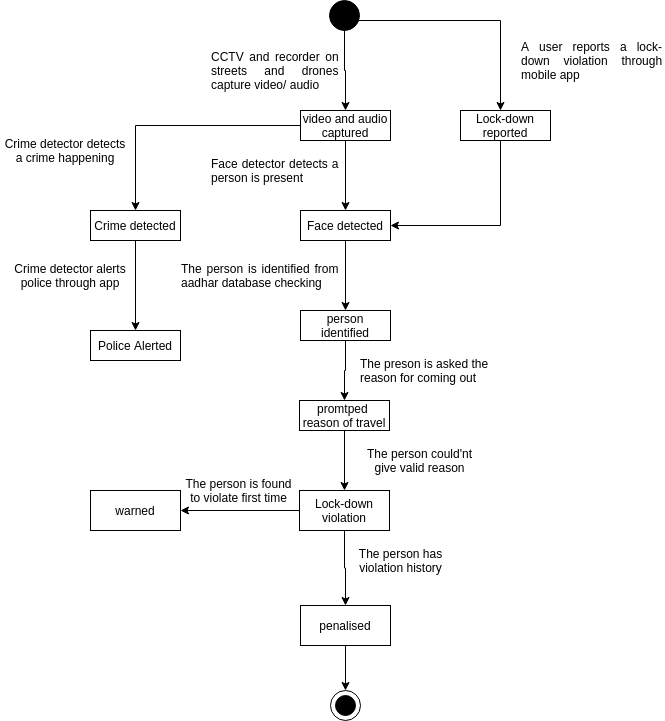
\includegraphics[height=.6\textwidth, width=.5\textwidth]{images/state_diagram.png} 

    \caption{State Diagram}
\end{figure}

 \begin{figure}
   \centering
\subfloat[Police's end]{   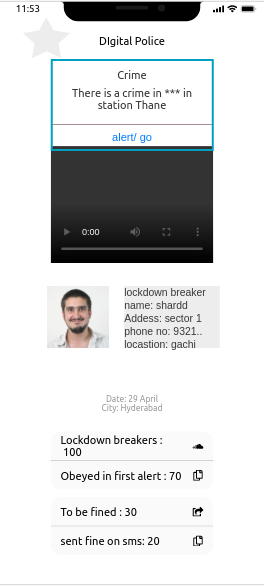
\includegraphics[height=.45\textwidth, width=.2\textwidth]{images/mobi.png}\label{fig:f1}} 
 
     \hfill
    \subfloat[Common person's end]{
    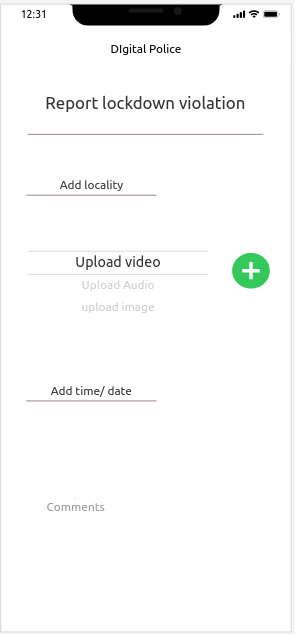
\includegraphics[height=.35\textwidth, width=.15\textwidth]{images/user_webapp.png} \label{fig:f2}
    }
    \caption{Web-app Interfaces}
  
\end{figure}


\section{Conclusion}
We thus designed a robust system "Digital police" with the help of face detection, drone surveillance, Natural language processing, signal processing for helping police ensure lock-down as well as law without actually going out in fields. The system uses drone and CCTV's deployed at various street locations to recognise the people who are seen out in lock-down and penalizes them by sending message of fine on mobile phone. The system not only helps ensure lock-down is not broken but also ensure safety by citing crimes as and when they are detected and alerting police. 


%-------------------------------------------------------------------------

{\small
\bibliographystyle{ieee}
\bibliography{egbib}
}

\end{document}
